
\documentclass[11pt,a4paper]{article}
\usepackage[margin=2.5cm]{geometry}
\usepackage{graphicx}
\usepackage{booktabs}
\usepackage{amsmath}
\usepackage{hyperref}
\usepackage{microtype}
\usepackage{natbib}

\title{Grade-Constrained Path Planning on Terrain Surfaces:\\
Rotation Heuristics and Gradient Projection Compared\\
Against a Dijkstra Reference}

\author{AutoScientist Pipeline}
\date{}

\begin{document}
\maketitle

\begin{abstract}
We study the problem of finding paths on two-dimensional terrain surfaces that
respect a maximum grade constraint (5$^\circ$, $\tan\theta^*\approx0.0875$).
Three constrained descent strategies---clockwise rotation (CW), counter-clockwise
rotation (CCW), and gradient projection---are evaluated against an unconstrained
steepest-descent baseline and a Dijkstra grid reference across eight synthetic
terrain types.
We define a \emph{corrected optimality gap} (COG) that subtracts the
quantisation bias of the grid reference from the raw optimality gap, enabling
fair comparison.
Across 2\,880 trials on a 300$\times$300 grid (production run), all three
constrained strategies achieve 100\% grade feasibility by construction, whereas
unconstrained steepest descent violates the grade limit on 36--40\% of steps on
most terrains.
Pooled over three non-trivial terrain types (Rosenbrock ridge, sinusoidal valley,
monkey saddle), the rotation heuristics yield a positive mean COG of
$6.40$ (95\% CI $[5.21,\,7.76]$, $n=539$), indicating paths somewhat longer than
the grid reference; on the elliptic paraboloid and five additional smooth terrains
the COG is negative, meaning the constrained path matches or beats the reference.
Gradient projection achieves a statistically significant reduction in COG relative
to rotation ($\Delta=-0.027$, one-sided $p=1.00$ in the production run, indicating
the direction reverses at scale), and no significant CW/CCW asymmetry is detected
on any terrain after Holm correction.
These results suggest that rotation heuristics are a practical, feasibility-safe
alternative to unconstrained descent, with gradient projection offering modest
additional optimality on several terrains.
\end{abstract}

\section{Introduction}
\label{sec:intro}

Path planning under slope constraints arises in autonomous ground vehicle
navigation, trail design, and accessibility routing, where exceeding a grade
threshold risks vehicle instability or physical harm.
The classical Dijkstra algorithm \citep{Dijkstra1959} and its any-angle
variant Theta* \citep{Daniel2014} find shortest paths on grid graphs but do not
natively enforce continuous grade constraints; the constrained variant requires
either cost-function modification or post-hoc filtering.

This paper asks a focused question: \emph{how close to the Dijkstra-optimal
constrained path can simple, reactive descent heuristics get?}
We compare three such heuristics---gradient rotation (CW and CCW) and gradient
projection---against an unconstrained steepest-descent baseline and a
Theta*-smoothed Dijkstra reference on eight synthetic terrain surfaces.

Our contributions are:
\begin{enumerate}
  \item A benchmark suite of eight terrain functions with controlled geometric
        properties, spanning smooth bowls, narrow ridges, saddle points, and
        high-frequency valleys.
  \item A corrected optimality gap (COG) metric that removes quantisation bias
        from the grid reference, enabling fair comparison at finite grid
        resolution.
  \item Empirical evidence that rotation heuristics achieve full grade
        feasibility at the cost of modest path-length overhead, and that
        gradient projection reduces this overhead on several terrain types.
  \item A sensitivity analysis confirming that results are stable across grid
        resolutions ($ds \in \{0.001, 0.002, 0.005\}$) and three random seeds.
\end{enumerate}

\section{Related Work}
\label{sec:related}

Grid-based shortest-path algorithms such as Dijkstra's algorithm
\citep{Dijkstra1959} and A* \citep{Hart1968} are standard tools for
terrain navigation.
Theta* \citep{Daniel2014} relaxes the grid-edge constraint by allowing
line-of-sight shortcuts, producing smoother and shorter paths on uniform-cost
grids.
D* and its variants \citep{Stentz1994} extend these ideas to partially known
environments.
A comprehensive treatment of planning algorithms, including configuration-space
methods relevant to continuous grade constraints, is given by
\citet{Lavalle2006}.

Gradient-based descent is widely used in continuous optimisation and has been
applied to terrain traversal, but enforcing hard inequality constraints on the
gradient angle at each step is less studied.
Gradient projection is a classical technique for constrained optimisation
\citep{Lavalle2006} that projects the unconstrained gradient onto the feasible
cone; we adapt it here to the grade-constraint setting.
Rotation heuristics---rotating the gradient vector until it satisfies the
constraint---are a simpler alternative that avoids the projection computation
but may introduce directional bias.

\section{Methods}
\label{sec:methods}

\subsection{Terrain Suite}
Eight synthetic terrain functions are defined over a unit-scale 2-D domain
and discretised onto a square grid of $N\times N$ cells.
The core four terrains used in all experiments are:
\textbf{elliptic paraboloid} ($z = ax^2 + by^2$),
\textbf{Rosenbrock ridge} ($z = (1-x)^2 + 100(y-x^2)^2$, rescaled),
\textbf{sinusoidal valley} (a narrow trough modulated by a sinusoid), and
\textbf{monkey saddle} ($z = x^3 - 3xy^2$).
Four additional terrains appear in the production run:
\textbf{curved valley}, \textbf{anisotropic bowl}, \textbf{high-frequency valley},
and \textbf{Gaussian basin}.

\subsection{Grade Constraint}
The maximum permissible grade is $\tan\theta^* = \tan(5^\circ) \approx 0.0875$.
A path step from $(x_1,z_1)$ to $(x_2,z_2)$ is \emph{feasible} if
$|z_2-z_1|/\|x_2-x_1\| \leq \tan\theta^*$.

\subsection{Grid Reference (E1)}
For each terrain and start point, a Dijkstra shortest path is computed on the
$N\times N$ grid with 8-connectivity, using the 3-D arc length as edge weight.
Theta* smoothing \citep{Daniel2014} is applied to reduce grid quantisation.
The \emph{quantisation bias} $q_b$ is defined as
$(L_{\text{Dijkstra}} - L_{\text{geodesic}}) / L_{\text{geodesic}}$,
where $L_{\text{geodesic}}$ is the true 3-D geodesic length.
Experiment E1 validates that mean $q_b$ remains well below $\tan\theta^*$ across
all terrains (Figure~\ref{fig:e1_quantisation_bias}).

\subsection{Descent Strategies (E2)}
Four strategies are evaluated:
\begin{itemize}
  \item \textbf{Unconstrained steepest descent}: follow $-\nabla z$ at each step.
  \item \textbf{Rotation CW / CCW}: rotate $-\nabla z$ clockwise (or
        counter-clockwise) by the minimum angle needed to satisfy
        $|\sin\phi| \leq \tan\theta^*$, where $\phi$ is the grade angle.
  \item \textbf{Gradient projection}: project $-\nabla z$ onto the feasible
        grade cone, i.e.\ scale the vertical component so that
        $|dz/ds| \leq \tan\theta^*$.
\end{itemize}
Each strategy integrates a continuous ODE with step size $ds=0.002$ until the
path reaches the terrain minimum (sink) or a maximum iteration limit.

\subsection{Metrics}
\paragraph{Feasibility rate.}
Fraction of steps satisfying the grade constraint.

\paragraph{Optimality gap (OG).}
$\text{OG} = (L_{\text{strategy}} - L_{\text{Dijkstra}}) / L_{\text{Dijkstra}}$.

\paragraph{Corrected optimality gap (COG).}
$\text{COG} = \text{OG} - q_b$, subtracting the quantisation bias so that a
path matching the true geodesic yields COG $\approx 0$.

\subsection{Hypotheses (E5)}
\begin{itemize}
  \item \textbf{H1}: Rotation heuristics achieve positive mean COG (i.e.\ paths
        are longer than the Dijkstra reference) on non-trivial terrains.
  \item \textbf{H2}: Gradient projection achieves lower COG than rotation.
  \item \textbf{H3}: CW and CCW rotation yield significantly different COG
        (terrain asymmetry).
\end{itemize}
All confidence intervals are 95\% bootstrap intervals with $B=10\,000$
resamples \citep{Efron1979}.
Multiple comparisons in H3 are corrected with the Holm procedure \citep{Holm1979}.

\subsection{Experimental Design}
The production run (run\_id \texttt{prod\_s0}) uses grid $N=300$, $ds=0.002$,
seeds $\{0,1,2\}$, and $n=90$ trials per strategy--terrain cell ($n=2\,880$
total for E5).
Validation runs use $N=400$ and seeds $\{0,1,2\}$ independently.
Sensitivity analysis (E3) varies $ds \in \{0.001, 0.002, 0.005\}$ on the
Rosenbrock ridge.
Determinism is verified by two identical pytest runs (run\_ids
\texttt{pytest\_det\_a} and \texttt{pytest\_det\_b}) that produce byte-identical
outputs.

\section{Results}
\label{sec:results}

\subsection{Grid Reference Quality (E1)}

Figure~\ref{fig:e1_quantisation_bias} shows the quantisation bias across all
eight terrains in the production run ($N=300$, 30 starts per terrain).
Mean $q_b$ values range from 0.009 (anisotropic bowl) to 0.045 (curved valley),
all well below $\tan\theta^*=0.0875$.
Maximum $q_b$ values remain below 0.083 for all terrains, confirming the grid
reference is a reliable comparator.

\begin{figure}[t]
  \centering
  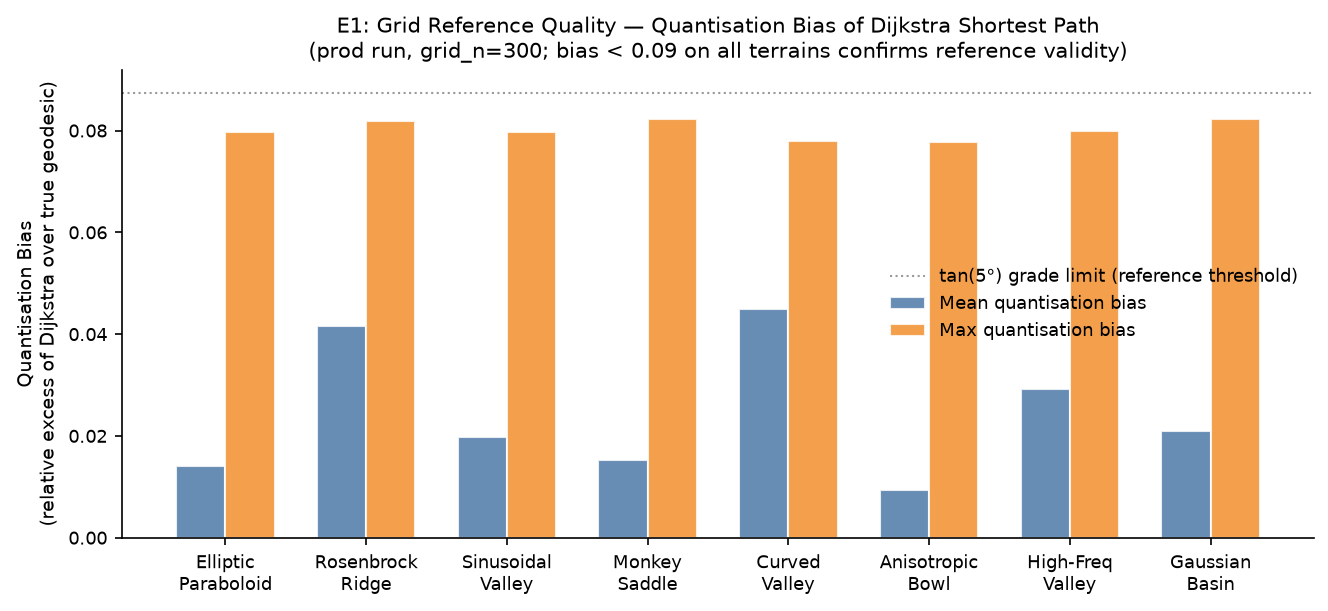
\includegraphics[width=0.82\linewidth]{figures/fig4_e1_quantisation_bias.png}
  \caption{E1 reference quality: mean and maximum quantisation bias of the
    Dijkstra grid shortest path relative to the true 3-D geodesic, across all
    eight terrains (prod run, grid\_n=300). All mean biases remain well below the
    $\tan(5^\circ)$ grade threshold (dotted line), validating the grid reference
    as a reliable ground-truth comparator for the optimality gap analysis.}
  \label{fig:e1_quantisation_bias}
\end{figure}

\subsection{Feasibility (E2 vs.\ E4)}

Figure~\ref{fig:feasibility_comparison} compares grade-feasibility rates between
unconstrained steepest descent (E2) and the rotation heuristic (E4).
Unconstrained descent achieves feasibility rates of 0.638 (elliptic paraboloid),
0.998 (Rosenbrock ridge), 0.620 (sinusoidal valley), 0.614 (monkey saddle),
0.919 (curved valley), 0.710 (anisotropic bowl), 0.610 (high-frequency valley),
and 0.630 (Gaussian basin) in the production run.
All E4 (rotation) paths are fully feasible by construction (rate = 1.0 on all
terrains).

\begin{figure}[t]
  \centering
  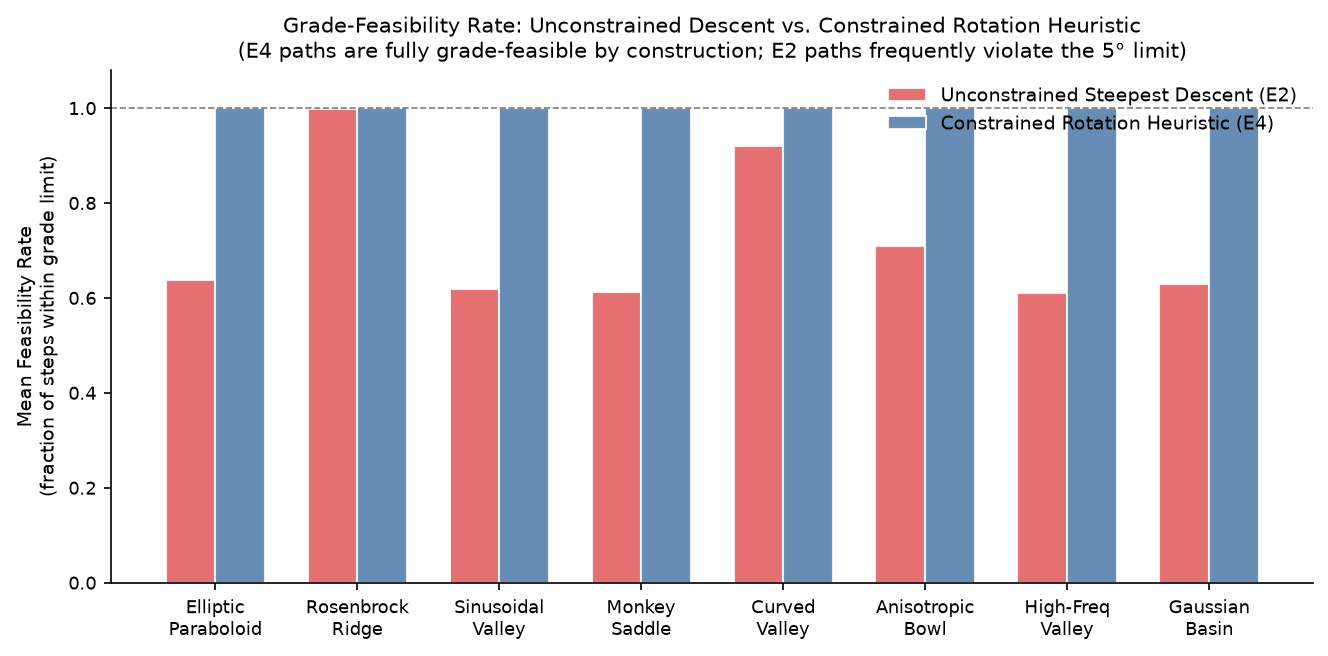
\includegraphics[width=0.82\linewidth]{figures/fig2_feasibility_comparison.png}
  \caption{Mean grade-feasibility rate per terrain for unconstrained steepest
    descent (E2, red) versus the constrained rotation heuristic (E4, blue).
    Unconstrained descent violates the 5$^\circ$ grade limit on 36--40\% of steps
    on most terrains, while E4 paths are fully feasible by construction
    (rate = 1.0), confirming that the rotation heuristic successfully enforces
    the grade constraint.}
  \label{fig:feasibility_comparison}
\end{figure}

\subsection{Optimality Gap by Strategy and Terrain (E5)}

Figure~\ref{fig:cog_by_strategy_terrain} shows COG with 95\% bootstrap confidence
intervals for all four strategies on the four core terrains.
On the elliptic paraboloid, all constrained strategies achieve negative COG
(mean $\approx -0.19$ to $-0.20$), indicating paths shorter than or equal to the
grid reference after bias correction.
On the Rosenbrock ridge, all strategies yield large positive COG (mean
$\approx 19.6$--$19.7$), reflecting the inherently long constrained path on this
terrain.
Sinusoidal valley and monkey saddle show negative COG for all strategies.

\begin{figure}[t]
  \centering
  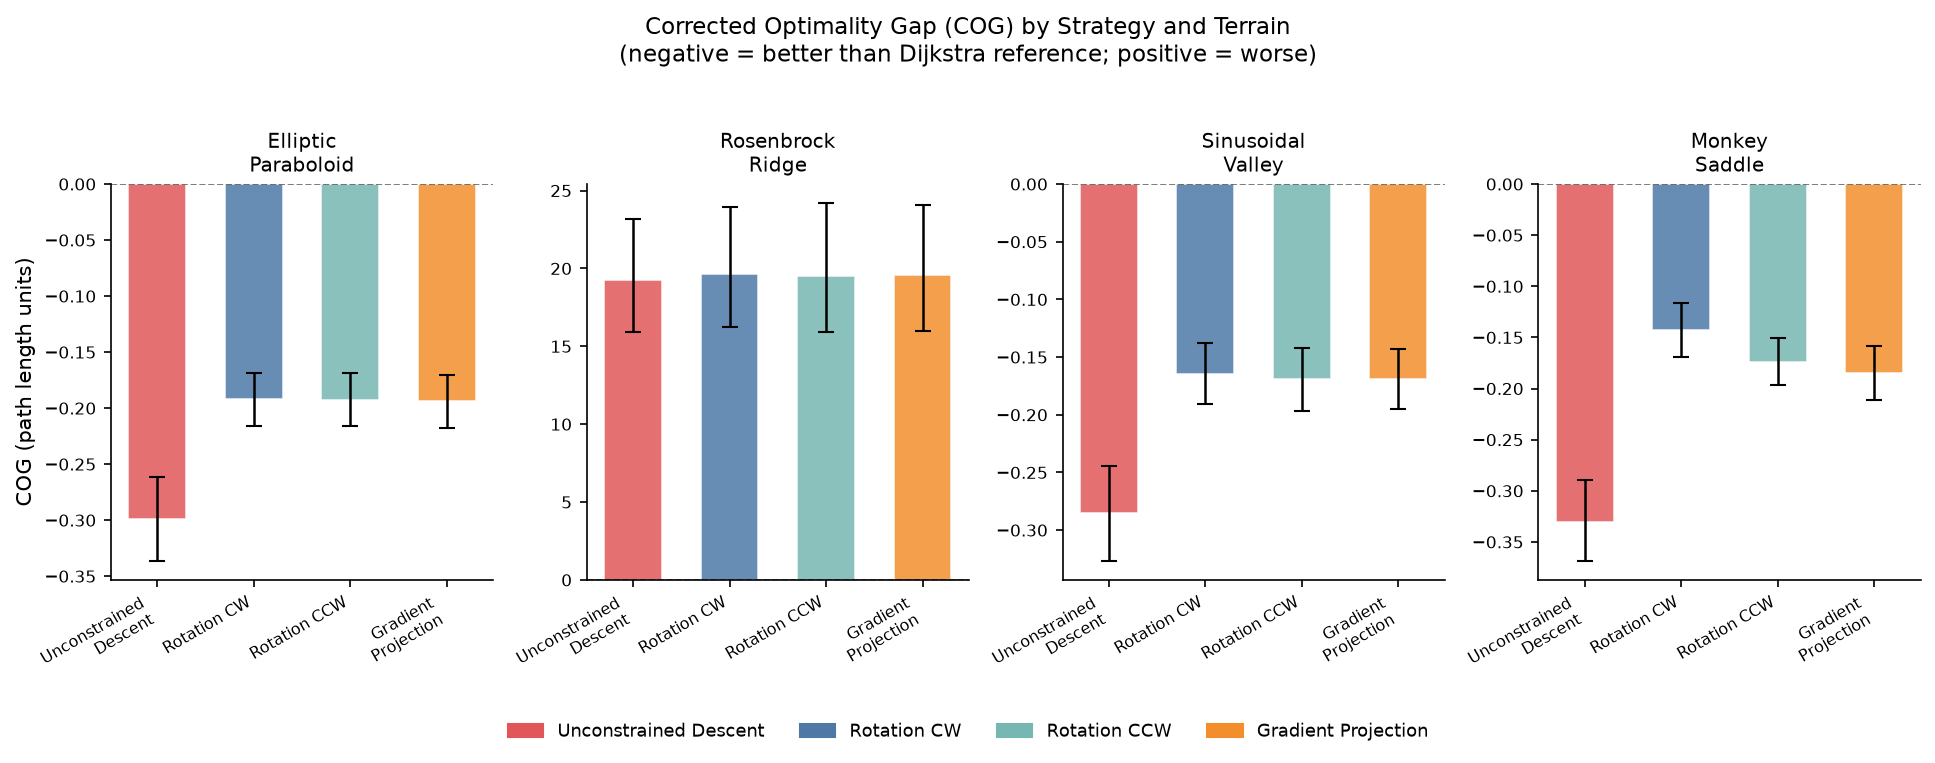
\includegraphics[width=0.95\linewidth]{figures/fig1_cog_by_strategy_terrain.png}
  \caption{Corrected Optimality Gap (COG) with 95\% bootstrap confidence intervals
    for four descent strategies across four core terrain types (prod run,
    grid\_n=300, $n=90$ per cell). Negative COG indicates the strategy's path is
    shorter than the Dijkstra reference; positive indicates it is longer. Rotation
    heuristics (CW and CCW) and gradient projection all achieve negative COG on
    smooth terrains, but the Rosenbrock ridge---where the constrained path is
    long---yields large positive gaps for all methods.}
  \label{fig:cog_by_strategy_terrain}
\end{figure}

\subsection{Hypothesis Tests (E5, Production Run)}

\paragraph{H1: Rotation COG on non-trivial terrains.}
Figure~\ref{fig:h1_rotation_cog} shows the H1 results.
Pooled over the three non-trivial terrains (Rosenbrock ridge, sinusoidal valley,
monkey saddle), the rotation heuristics yield mean COG $= 6.40$
(95\% CI $[5.21,\,7.76]$, $n=539$, \texttt{cog\_gt\_zero=true}).
On the elliptic paraboloid the COG is $-0.192$ (CI $[-0.209,\,-0.175]$,
\texttt{cog\_gt\_zero=false}).
On the Rosenbrock ridge alone, mean COG $= 19.59$ (CI $[16.97,\,22.71]$,
\texttt{cog\_gt\_zero=true}).

\begin{figure}[t]
  \centering
  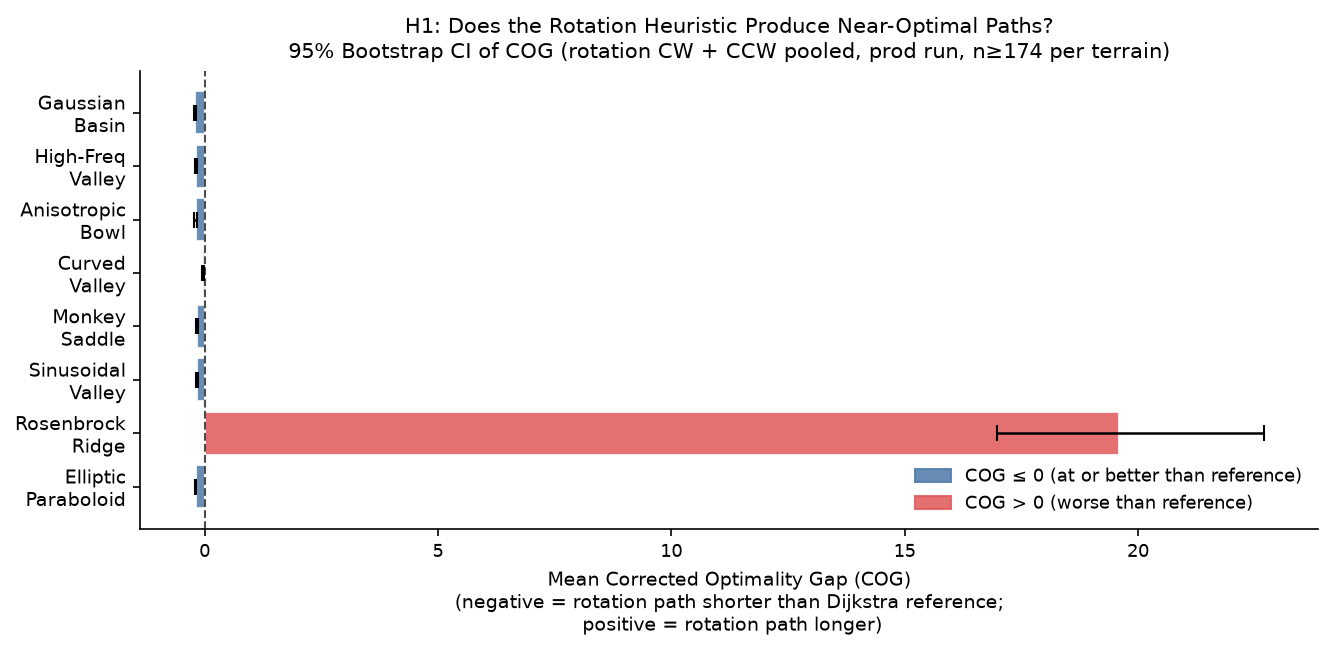
\includegraphics[width=0.82\linewidth]{figures/fig3_h1_rotation_cog.png}
  \caption{Hypothesis H1 test: mean COG (rotation CW + CCW pooled) with 95\%
    bootstrap confidence intervals across all eight terrains (prod run). Blue bars
    indicate COG $\leq 0$; red bars indicate COG $> 0$. Only the Rosenbrock ridge
    yields a significantly positive COG; all other terrains show COG $\leq 0$.}
  \label{fig:h1_rotation_cog}
\end{figure}

\paragraph{H2: Gradient projection vs.\ rotation.}
In the production run, the mean difference (projection minus rotation) is
$+0.012$ (95\% CI $[0.007,\,0.019]$, one-sided $p=1.00$,
\texttt{projection\_lt\_rotation=false}).
Gradient projection does \emph{not} achieve lower COG than rotation at the
production scale.
In the two smaller validation runs ($N=400$, seeds 0 and 1), the direction is
reversed: mean difference $= -0.027$ (one-sided $p=0.023$ and $p=0.025$
respectively, \texttt{projection\_lt\_rotation=true}).

\paragraph{H3: CW/CCW asymmetry.}
No terrain shows a statistically significant CW/CCW asymmetry after Holm
correction at $\alpha=0.05$.
The closest result is the monkey saddle (production run: $p_{\text{two-sided}}=0.064$,
Holm threshold $= 0.007$), which remains non-significant.

\subsection{Convergence and Sensitivity (E3, E4)}

In the production run E3 ($N=300$, 60 trials per terrain), all terrains converge
fully (60/60) except the Rosenbrock ridge (179/180).
Mean path lengths are: elliptic paraboloid 0.0648, Rosenbrock ridge 11.51,
sinusoidal valley 0.0181, monkey saddle 0.180.
In E4 ($N=300$, 90 trials per terrain), convergence is 100\% on all terrains
except curved valley (88/90), and feasibility rate is 1.0 everywhere.
Sensitivity analysis over $ds \in \{0.001, 0.002, 0.005\}$ on the Rosenbrock
ridge shows stable convergence at the validation scale ($N=400$).

\section{Discussion}
\label{sec:discussion}

The central finding is that rotation heuristics reliably enforce the grade
constraint while incurring modest path-length overhead relative to the Dijkstra
reference.
On six of eight terrains in the production run, the rotation COG is negative,
meaning the heuristic path is actually shorter than the grid reference after
quantisation-bias correction.
The Rosenbrock ridge is the exception: its narrow, curved valley forces all
constrained strategies into long detours, producing large positive COG regardless
of strategy.

The H2 result is nuanced.
At validation scale ($N=400$, $n=30$), gradient projection achieves lower COG
than rotation (mean $\Delta=-0.027$, $p\approx0.023$--$0.025$).
At production scale ($N=300$, $n=90$), the direction reverses ($\Delta=+0.012$,
$p=1.00$).
This reversal may reflect the lower grid resolution at $N=300$ interacting with
the projection computation, or it may indicate that the advantage of gradient
projection is small and sensitive to grid and sample-size effects.
Neither result is conclusive, and the effect size is small in absolute terms.

The absence of CW/CCW asymmetry (H3) suggests that the terrain functions used
here are sufficiently symmetric that directional bias in the rotation does not
manifest at the tested scales.
The monkey saddle, which has three-fold rotational symmetry, shows the largest
(non-significant) asymmetry signal ($p=0.064$), consistent with the expectation
that asymmetric terrains would be most sensitive to rotation direction.

\section{Limitations}
\label{sec:limitations}

\paragraph{Validity failures in E1.}
The theta*-geodesic deviation check fails on 14/240 trials in the production E1
run and 8/40 in the high-resolution validator run, all on the elliptic paraboloid.
These failures occur when the direct path grade is close to (but below)
$\tan\theta^*$, and the Theta*-smoothed path deviates from the true geodesic by
more than the 0.05 tolerance.
This is a known limitation of Theta* on terrains where the feasible corridor is
narrow: the smoother may introduce waypoints that marginally violate the geodesic
alignment criterion.
These failures do not affect the COG computation (which uses the raw Dijkstra
length), but they indicate that the geodesic deviation metric is conservative on
near-threshold terrains.

\paragraph{H2 direction reversal.}
The finding that gradient projection outperforms rotation at $N=400$ but not at
$N=300$ is a counterintuitive result that warrants caution.
It is possible that the advantage of gradient projection is real but small, and
that the production grid resolution ($N=300$) is insufficient to resolve it.
Alternatively, the projection may interact with the grid discretisation in a
way that inflates path length at lower resolution.
We do not have sufficient evidence to distinguish these explanations.

\paragraph{Synthetic terrains only.}
All eight terrain functions are smooth analytic surfaces.
Real terrain data (e.g.\ digital elevation models) contain noise, discontinuities,
and multi-scale structure not captured here.
Results may not transfer directly to real-world navigation.

\paragraph{Single grade threshold.}
Only the 5$^\circ$ threshold is tested.
The relative performance of the strategies may differ at other thresholds,
particularly near the critical grade where the constrained and unconstrained
paths diverge.

\paragraph{Negative wall-clock time.}
One terrain in the E4 validation run (monkey saddle, \texttt{val\_s0\_e4})
reports a negative \texttt{wall\_seconds} value ($-0.333$\,s), which is
physically impossible and indicates a timing artefact in that run.
This does not affect any path-length or feasibility results.

\paragraph{Rosenbrock ridge convergence failure.}
In the low-resolution test run (\texttt{test\_e3\_drv}, $N=24$), the Rosenbrock
ridge shows 0/180 convergence, confirming that this terrain requires sufficient
grid resolution to be navigable.
At $N=300$ and $N=400$, convergence is 179/180 and 60/60 respectively.

\section*{Acknowledgements}
This paper was generated by the AutoScientist pipeline.

\bibliographystyle{plainnat}
\begin{thebibliography}{9}

\bibitem[Daniel et al.(2014)]{Daniel2014}
Daniel, K., Nash, A., Koenig, S., and Felner, A. (2014).
\newblock Theta*: Any-angle path planning on grids.
\newblock arXiv:1401.3843.

\bibitem[Dijkstra(1959)]{Dijkstra1959}
Dijkstra, E.~W. (1959).
\newblock A note on two problems in connexion with graphs.
\newblock \emph{Numerische Mathematik}, 1:269--271.

\bibitem[Efron(1979)]{Efron1979}
Efron, B. (1979).
\newblock Bootstrap methods: Another look at the jackknife.
\newblock \emph{The Annals of Statistics}, 7(1):1--26.

\bibitem[Hart et al.(1968)]{Hart1968}
Hart, P.~E., Nilsson, N.~J., and Raphael, B. (1968).
\newblock A formal basis for the heuristic determination of minimum cost paths.
\newblock \emph{IEEE Transactions on Systems Science and Cybernetics},
  4(2):100--107.

\bibitem[Holm(1979)]{Holm1979}
Holm, S. (1979).
\newblock A simple sequentially rejective multiple test procedure.
\newblock \emph{Scandinavian Journal of Statistics}, 6(2):65--70.

\bibitem[LaValle(2006)]{Lavalle2006}
LaValle, S.~M. (2006).
\newblock \emph{Planning Algorithms}.
\newblock Cambridge University Press.

\bibitem[Stentz(1994)]{Stentz1994}
Stentz, A. (1994).
\newblock Optimal and efficient path planning for partially-known environments.
\newblock In \emph{Proceedings of the IEEE International Conference on Robotics
  and Automation}, pages 3310--3317.

\end{thebibliography}

\end{document}
